\documentclass{scrartcl}
\usepackage[utf8]{inputenc}
\usepackage[english]{babel} % Trennung nach der neuen deutschen Rechtschreibung
\usepackage[utf8]{inputenc}
\usepackage[T1]{fontenc}
\usepackage{lmodern}

\usepackage{amsmath} % Erweiterte Mathematik-Umgebung
\usepackage{amsfonts} % zusätzliche Mathematik-Schrifttypen (v.a. \mathbb für Mengen)
\usepackage{ulem}

\usepackage{graphics}%soll beim Graphiken einfügen hilfreich sein
\usepackage{graphicx}
\usepackage{wrapfig}%lässt Textumflossene Bildeinbindung zu
\usepackage{epstopdf}%soll eps in pdf umwandeln

\usepackage[a4paper, portrait, margin=2.5cm]{geometry}

\titlehead{\centering University of Luxemburg}
\subject{Travaux Pratiques}
\title{Surface Tension}
\subtitle{Joana Ferreira}
\date{TP Session 19/11/2021}
\author{Louis-Hendrik Barboutie (020157041C)\\ Frederik Ehl (0201719742) \\ Florence Schmerber (0201845640)}

\begin{document}

\maketitle

\clearpage

\tableofcontents
\listoffigures
	
\clearpage

\section{Introduction}
In this experiment our goal is to determine the surface tension of different mixtures of ethanol with water at different concentrations. We will be using two different methods. We begin with the Ring method, also called the Du Nouy method, and then Jaerger's Method, which makes use of the bubble pressure method. Finally we want to compare our experimental values with the literature ones to determine the accuracy of the two different methods.

\section{Ring Method}
\subsection{Experimental setup}

In this first experiment the setup consists of a metal ring with a diameter of $6cm$, which is attached to the bottom side of a balance. The ring is then immersed into a Petri dish filled with the liquid under examination.
The Petri dish is standing on top of a lab jack, which is used to carefully lower the the Petri dish. 

\begin{figure}[h]
    \centering
    \includegraphics[width=10cm]{1637334165537.jpg}
    \caption{Setup for the ring method}
    \label{fig:1}
\end{figure}


\subsection{Realization}
First of all we make sure, that the balance is evened. We then fill the Petri dish with the liquid to analyze and attach the metal ring to the hook hanging from the bottom of the balance. This has to be done with gloves, in order to avoid a film of fat both on the ring and in the Petri dish, which would falsify the results. We then carefully immerse the ring horizontally into the liquid. We then lower the lab jack, which is equivalent to pulling up the ring but avoids vibrations. Due to the surface tension of the liquid, it is pulled up by the ring, which requires a certain force. What we actually measure is the weight of the solution amount we are pulling up, and deduce the force with the relation $F = m \cdot g_0$. The surface tension is then given by $\sigma = \frac{F}{4 \pi R}$, where $R$ is the radius of the ring.
This method will be repeated with different concentrations of ethanol in water, i.e. $0\%, 25\%, 50\%, 75\%$ and $100\%$ ethanol solutions.

\medskip

\textit{Remark: the ring couldn't be evenly submerged in the solution. The cause could be the unevenness of the lab jack on the table.}

\newpage

\subsection{Results}

We use the average values in order to reduce the systematic error.

\begin{figure}[h]
    \centering
    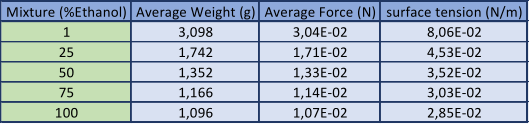
\includegraphics{Mappe1.png}
    \caption{Measured values}
    \label{fig:2}
\end{figure}

\begin{figure}[htbp]
    \centering
    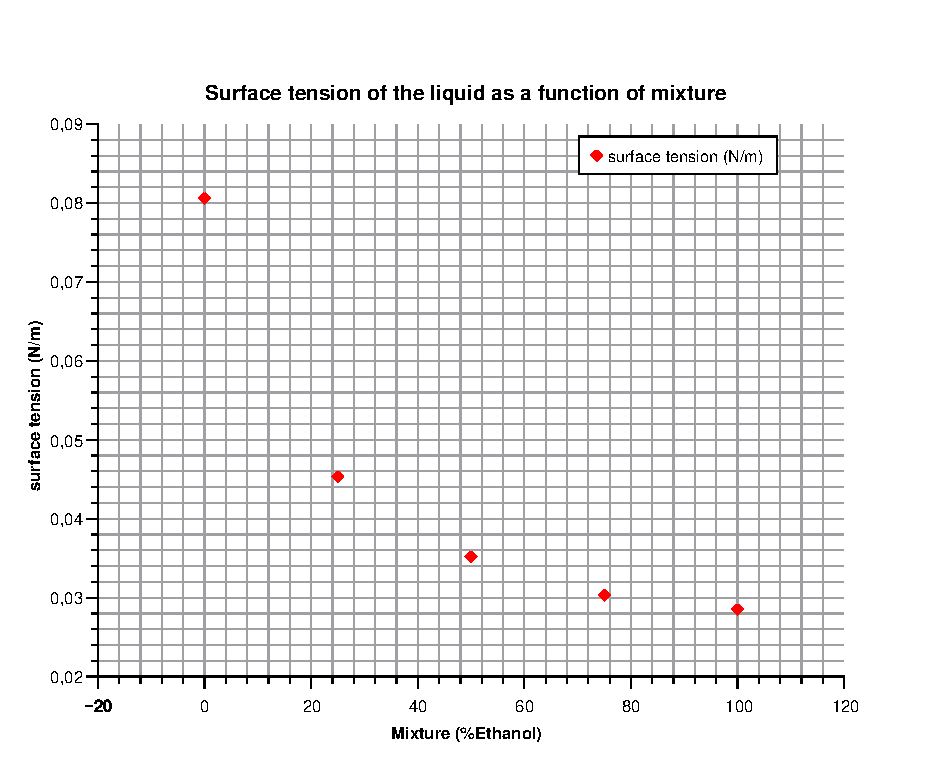
\includegraphics[width=12cm]{RingMethodSurfaceTension.eps}
    \caption{Ring method: surface tension as a function of the mixture}
    \label{fig:3}
\end{figure}

We can then compute our relative error for pure water and pure ethanol to the literature data:

\begin{equation}
    \frac{|\sigma_{water,theoretical}-\sigma_{water,experimental}|}{\sigma_{water,theoretical}} \cdot 100 \approx 12 \%
\end{equation}

\begin{equation}
    \frac{|\sigma_{ethanol,theoretical}-\sigma_{ethanol,experimental}|}{\sigma_{ethanol,theoretical}} \cdot 100 \approx 30 \%
\end{equation}

Our values deviate significantly from the literature ones, but it's to be expected, since we couldn't guarantee a vibe-free environment, and had to trust the ratio labels of our solutions.

\section{Jaeger's Method}
\subsection{Experimental setup}

In this second experiment we will be using a construction consisting of a Woulff bottle, a capillary immersed into a liquid and a differential manometer, all connected via a tube. Dropping Water drops into the Woulff bottle creates an overpressure, since the air inside the bottle is replaced by the water. This overpressure is transferred to the capillary. The connected differential manometer determines the difference of pressure $\Delta p$ between the pressure inside the capillary and the atmospheric pressure.

\begin{figure}[h]
   \centering
    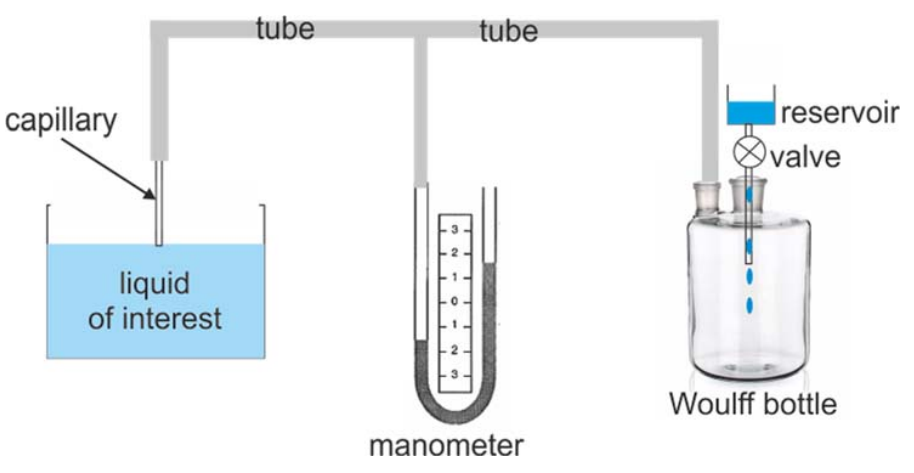
\includegraphics[scale=0.5]{TP6_Setup_Jaergers_Method.PNG}
    \caption{Experimental setup Jaeger's method}
    \label{fig:4}
\end{figure}



\subsection{Realization}
In order to determine the surface tension of the liquid in question, we make use of the bubble pressure method. The created overpressure $\Delta p$ is utilized to force a gas bubble out of the capillary vertically immersed into the liquid. 
On the manometer, we read the maximum pressure before the bubble comes out of the capillary. We note the difference of initial and maximum pressure as $\Delta k$. The dimension of $\Delta k$ is not important, since we're using a relative method. As before, we do 5 measurements for each ratio between water and ethanol:$0\%, 25\%, 50\%, 75\%$ and $100\%$.

Using the relation:

\centering
\begin{equation}
    \frac{\sigma_{mixture}}{\sigma_{water}}=\frac{\Delta p_{mixture}}{\Delta p_{water}}=\frac{\Delta k_{mixture}}{\Delta k_{water}}\nonumber
\end{equation}
\flushleft
\medskip

 Where water is used as calibrating substance, i.e. we take the literature value of $\sigma_{water}=7.2\cdot10^{-2} N/m$. So in order to determine the surface tension of the liquid in question we simply use:
 
 \centering
 \begin{equation}
     \sigma_{mixture}=\frac{\Delta k_{mixture}}{\Delta k_{water}}\sigma_{water}
 \end{equation}
 \flushleft

\newpage

\subsection{Results}

For $\Delta k$ we obtained the following values for the different solutions:

\begin{figure}[h]
    \centering
    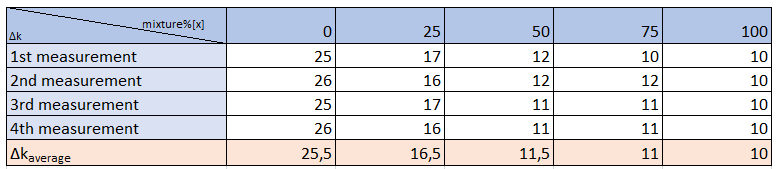
\includegraphics[width=15cm]{TP6_Delta_K_Ring_method.PNG}
    \caption{Table of measured k values}
    \label{fig:5}
\end{figure}

 For accuracy we will be using the value of $\Delta k_{average}$ for our calculations of $\sigma_{mixture}$.

\begin{figure}[h]
    \centering
    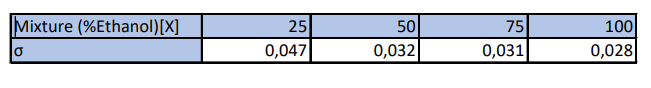
\includegraphics[width=15cm]{TP6_Sigma_Ring_Method.PNG}
    \caption{Table of $\sigma$ values}
    \label{fig:6}
\end{figure}

 We can observe that the bigger the ratio of ethanol, the smaller the capillary pressure and therefore the surface tension decreases with increasing concentration of ethanol in the solution.

\begin{figure}[h]
    \centering
    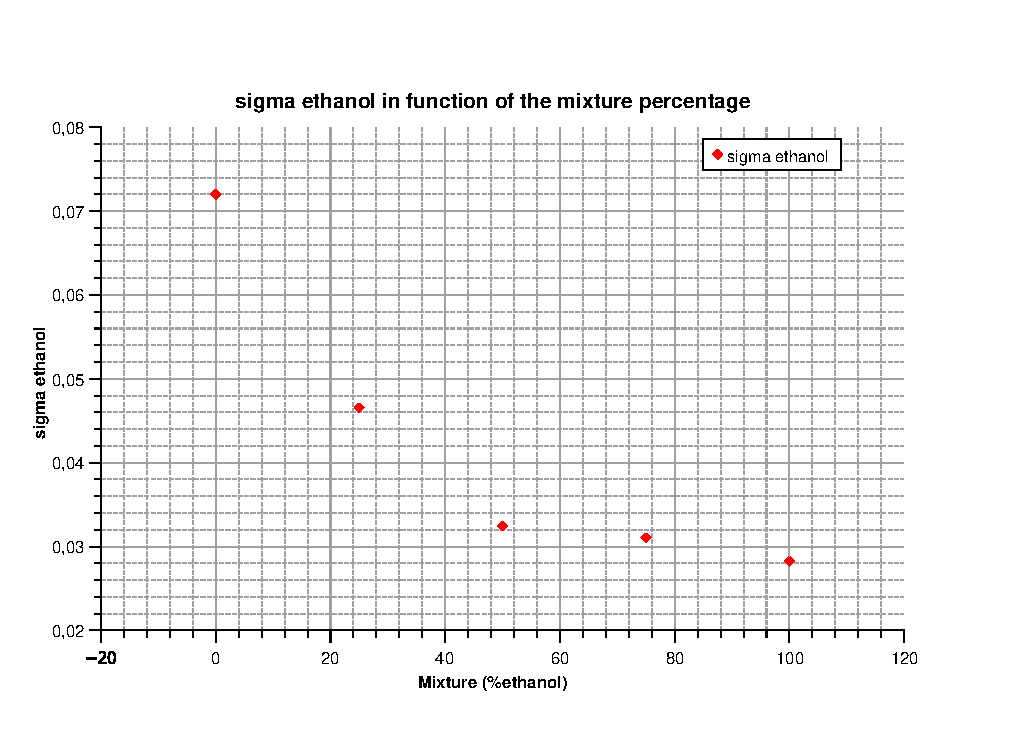
\includegraphics[width=12cm]{BubbleMethodSigmaEthanol.eps}
    \caption{Jaeger method: surface tension of ethanol as a function of the mixture}
    \label{fig:7}
\end{figure}

Relative error for pure ethanol:

\begin{equation}
    \frac{|\sigma_{ethanol,theoretical}-\sigma_{ethanol,experimental}|}{\sigma_{ethanol,theoretical}} \cdot 100 \approx 27 \%
\end{equation}


\section{Conclusion}
With our measurements we can conclude that the surface tension of water is in fact bigger than the one for ethanol. For the first method, the ring method that consists of measuring the force acting on the surface of the solution, we get a deviation of $30\%$ from the literature value. For the Jaeger method, for which we measured $\Delta k$, which is related to the difference of the pressure shown on the manometer, we get once more a deviation of $27\%$. Both methods aren't precise enough to get an exact value for the surface tension of ethanol. Especially for the Jaeger method, it was hard to read the values because when the ratio of ethanol got bigger, the manometer began to oscillate around the reading value.

\end{document}
